\documentclass[9pt,hyperref={pdfpagemode=FullScreen,urlcolor=blue},xcolor=x11names]{beamer}

\mode<presentation>
{
  \usetheme{Warsaw}
  %\usetheme{Darmstadt}
  %\usetheme{Marburg}
  \setbeamertemplate{navigation symbols}{}

  %\usecolortheme{crane}
  %\usecolortheme{rose,sidebartab}

  \usecolortheme{beaver}
  %\usecolortheme{lily,sidebartab}
  %\usecolortheme{seahorse}

  \usefonttheme{serif}

  \setbeamertemplate{footline}[page number]
  \setbeamertemplate{sidebar canvas right}[vertical shading][top=palette
  primary.bg,%,middle=white,
  bottom=palette primary.bg]
  %\setbeamertemplate{sections/subsections in toc}[section numbered,subsection numbered]

  %\setbeamertemplate{itemize subitem}[circle]

  \setbeamercovered{transparent}

  %\beamertemplatenavigationsymbolsempty

  \useinnertheme{default}
}

\usepackage[utf8]{inputenc}
\usepackage[T1]{fontenc}
\usepackage{lmodern}
\usepackage{xspace}
\usepackage{amsmath,amssymb}
\usepackage[english]{babel}
%\usepackage[latin1]{inputenc}
%\usepackage[T1]{fontenc}
\usepackage{aeguill,fourier}

% souligne, barre
\usepackage{ulem}
%\usepackage[x11names]{xcolor}

\usepackage{pgf,pgfarrows,pgfnodes,pgfautomata,pgfheaps,pgfshade}


\usepackage{wasysym}
\usepackage{fancyvrb}
%\usepackage{verbatim}
\usepackage{marvosym}

\usepackage{colortbl}

\usepackage{pdftricks}
\begin{psinputs}
\usepackage{pstricks}
\usepackage{pst-bar}
\usepackage{pstricks-add}
\end{psinputs}

\usepackage{ulem}

\usepackage{ifdraft}
\usepackage{animate}
\usepackage{multimedia}

%\usepackage{texmath}

\usepackage{tikz}
\usetikzlibrary{calc}
\usetikzlibrary{patterns}   % for hatching
\usetikzlibrary{positioning}
\usetikzlibrary{decorations.pathreplacing}
\usetikzlibrary{decorations.pathmorphing}
\usetikzlibrary{arrows, decorations.markings}
\usetikzlibrary{shapes.geometric}
\newcommand{\warningsign}{\tikz[baseline=-.75ex] \node[shape=regular polygon, regular polygon sides=3, inner sep=0pt, draw, thick] {\textbf{!}};}
\newcommand{\reddanger}{\textcolor{red}{\danger}}


% the following is from 
% http://tex.stackexchange.com/questions/4811/make-first-row-of-table-all-bold
%\usepackage{array}
%\newcolumntype{$}{>{\global\let\currentrowstyle\relax}}
%\newcolumntype{^}{>{\currentrowstyle}}
%\newcommand{\rowstyle}[1]{\gdef\currentrowstyle{#1}%
%  #1\ignorespaces
%}

\usepackage{listings}
\usepackage{minted}

\usepackage{caption}


%%%%%%%%%%%%%%%%%%%
\hypersetup{%
  pdftitle={PATC-KOKKOS-2017},%
  pdfauthor={Pierre Kestener - CEA Saclay - MDLS - http://www.maisondelasimulation.fr},
  pdfsubject={Introdcution to Kokkos},
  pdfkeywords={KOKKOS, C++, GPU},
  pdfproducer={pdflatex avec la classe BEAMER},
  bookmarksopen=false,
  urlcolor=blue
}

%%%%%%%%%%%%%%%%%%%%%%%%%%%%%%%%%%%%%%%%%%%%%%%%%%%%%%%%%%%%%%%
%%%%%%%%%%%%%%%%%%%%%%%%%%%%%%%%%%%%%%%%%%%%%%%%%%%%%%%%%%%%%%%
%%%%%%%%%%%%%%%%%%%%%%%%%%%%%%%%%%%%%%%%%%%%%%%%%%%%%%%%%%%%%%%

\title{Kokkos, Modern C++, performance portability, ...}

\author
{
  \mbox{\underline{Pierre Kestener}}\inst{1}
}

\institute[mdls sap]{%
  \inst{1}%
  CEA Saclay, DSM, Maison de la Simulation
}

\date{PATC, January, 16-18th, 2017}

\pgfdeclareimage[height=0.5cm]{university-logo}{./images/Sigle-mdls}
\logo{\pgfuseimage{university-logo}}


%%%%%%%%%%%%%%%%%%%%%
\pgfdeclareimage[width=2.0cm]{sigle-cea}{./images/Sigle-mdls}
\pgfdeclareimage[width=2.0cm]{sigle-prace}{images/logo_prace}
\pgfdeclareimage[width=2.0cm]{sigle-nvidia}{images/NV_CUDA_Teaching_Center_3D.jpg}

\titlegraphic{
  % \pgfuseimage{sigle-prace}
  \hfill
  \pgfuseimage{sigle-cea}
  \hfill
  % \pgfuseimage{sigle-nvidia}
}



\begin{document}


\definecolor{green2}{rgb}{0.1,0.8,0.1} 
\definecolor{trust}{rgb}{0.71,0.14,0.07}
\definecolor{FancyPurple}{rgb}{0.5176, 0.1137, 0.2314}

\colorlet{redshaded}{red!25!bg}
\colorlet{shaded}{black!25!bg}
\colorlet{shadedshaded}{black!10!bg}
\colorlet{blackshaded}{black!40!bg}

\colorlet{darkred}{red!80!black}
\colorlet{darkblue}{blue!80!black}
\colorlet{darkgreen}{green!70!black}
\colorlet{greenshaded}{green!95!bg}
%\colorlet{coral}{Coral1!95!bg}

%red, green, blue, cyan, magenta, yellow, black, white, darkgray, gray,
%lightgray, brown, lime, olive, orange, pink, purple, teal, violet

\newcommand\myurl[1]{\textcolor{purple}{\underline{\url{#1}}}}
\newcommand\myhref[2]{\textcolor{purple}{\underline{\href{#1}{#2}}}}

\newcommand\mySmiley{\textcolor{darkgreen}{\Smiley{}}}
\newcommand\myFrowny{\textcolor{red}{\Frowny{}}}

%% Big-O notation.
\providecommand{\OO}[1]{\ensuremath{\operatorname{O}\bigl(#1\bigr)}}

% definition des couleurs pour affichage de code
\makeatletter
\def\PY@reset{\let\PY@it=\relax \let\PY@bf=\relax%
    \let\PY@ul=\relax \let\PY@tc=\relax%
    \let\PY@bc=\relax \let\PY@ff=\relax}
\def\PY@tok#1{\csname PY@tok@#1\endcsname}
\def\PY@toks#1+{\ifx\relax#1\empty\else%
    \PY@tok{#1}\expandafter\PY@toks\fi}
\def\PY@do#1{\PY@bc{\PY@tc{\PY@ul{%
    \PY@it{\PY@bf{\PY@ff{#1}}}}}}}
\def\PY#1#2{\PY@reset\PY@toks#1+\relax+\PY@do{#2}}

\def\PY@tok@gd{\def\PY@tc##1{\textcolor[rgb]{0.63,0.00,0.00}{##1}}}
\def\PY@tok@gu{\let\PY@bf=\textbf\def\PY@tc##1{\textcolor[rgb]{0.50,0.00,0.50}{##1}}}
\def\PY@tok@gt{\def\PY@tc##1{\textcolor[rgb]{0.00,0.25,0.82}{##1}}}
\def\PY@tok@gs{\let\PY@bf=\textbf}
\def\PY@tok@gr{\def\PY@tc##1{\textcolor[rgb]{1.00,0.00,0.00}{##1}}}
\def\PY@tok@cm{\let\PY@it=\textit\def\PY@tc##1{\textcolor[rgb]{0.25,0.50,0.50}{##1}}}
\def\PY@tok@vg{\def\PY@tc##1{\textcolor[rgb]{0.10,0.09,0.49}{##1}}}
\def\PY@tok@m{\def\PY@tc##1{\textcolor[rgb]{0.40,0.40,0.40}{##1}}}
\def\PY@tok@mh{\def\PY@tc##1{\textcolor[rgb]{0.40,0.40,0.40}{##1}}}
\def\PY@tok@go{\def\PY@tc##1{\textcolor[rgb]{0.50,0.50,0.50}{##1}}}
\def\PY@tok@ge{\let\PY@it=\textit}
\def\PY@tok@vc{\def\PY@tc##1{\textcolor[rgb]{0.10,0.09,0.49}{##1}}}
\def\PY@tok@il{\def\PY@tc##1{\textcolor[rgb]{0.40,0.40,0.40}{##1}}}
\def\PY@tok@cs{\let\PY@it=\textit\def\PY@tc##1{\textcolor[rgb]{0.25,0.50,0.50}{##1}}}
\def\PY@tok@cp{\def\PY@tc##1{\textcolor[rgb]{0.74,0.48,0.00}{##1}}}
\def\PY@tok@gi{\def\PY@tc##1{\textcolor[rgb]{0.00,0.63,0.00}{##1}}}
\def\PY@tok@gh{\let\PY@bf=\textbf\def\PY@tc##1{\textcolor[rgb]{0.00,0.00,0.50}{##1}}}
\def\PY@tok@ni{\let\PY@bf=\textbf\def\PY@tc##1{\textcolor[rgb]{0.60,0.60,0.60}{##1}}}
\def\PY@tok@nl{\def\PY@tc##1{\textcolor[rgb]{0.63,0.63,0.00}{##1}}}
\def\PY@tok@nn{\let\PY@bf=\textbf\def\PY@tc##1{\textcolor[rgb]{0.00,0.00,1.00}{##1}}}
\def\PY@tok@no{\def\PY@tc##1{\textcolor[rgb]{0.53,0.00,0.00}{##1}}}
\def\PY@tok@na{\def\PY@tc##1{\textcolor[rgb]{0.49,0.56,0.16}{##1}}}
\def\PY@tok@nb{\def\PY@tc##1{\textcolor[rgb]{0.00,0.50,0.00}{##1}}}
\def\PY@tok@nc{\let\PY@bf=\textbf\def\PY@tc##1{\textcolor[rgb]{0.00,0.00,1.00}{##1}}}
\def\PY@tok@nd{\def\PY@tc##1{\textcolor[rgb]{0.67,0.13,1.00}{##1}}}
\def\PY@tok@ne{\let\PY@bf=\textbf\def\PY@tc##1{\textcolor[rgb]{0.82,0.25,0.23}{##1}}}
\def\PY@tok@nf{\def\PY@tc##1{\textcolor[rgb]{0.00,0.00,1.00}{##1}}}
\def\PY@tok@si{\let\PY@bf=\textbf\def\PY@tc##1{\textcolor[rgb]{0.73,0.40,0.53}{##1}}}
\def\PY@tok@s2{\def\PY@tc##1{\textcolor[rgb]{0.73,0.13,0.13}{##1}}}
\def\PY@tok@vi{\def\PY@tc##1{\textcolor[rgb]{0.10,0.09,0.49}{##1}}}
\def\PY@tok@nt{\let\PY@bf=\textbf\def\PY@tc##1{\textcolor[rgb]{0.00,0.50,0.00}{##1}}}
\def\PY@tok@nv{\def\PY@tc##1{\textcolor[rgb]{0.10,0.09,0.49}{##1}}}
\def\PY@tok@s1{\def\PY@tc##1{\textcolor[rgb]{0.73,0.13,0.13}{##1}}}
\def\PY@tok@sh{\def\PY@tc##1{\textcolor[rgb]{0.73,0.13,0.13}{##1}}}
\def\PY@tok@sc{\def\PY@tc##1{\textcolor[rgb]{0.73,0.13,0.13}{##1}}}
\def\PY@tok@sx{\def\PY@tc##1{\textcolor[rgb]{0.00,0.50,0.00}{##1}}}
\def\PY@tok@bp{\def\PY@tc##1{\textcolor[rgb]{0.00,0.50,0.00}{##1}}}
\def\PY@tok@c1{\let\PY@it=\textit\def\PY@tc##1{\textcolor[rgb]{0.25,0.50,0.50}{##1}}}
\def\PY@tok@kc{\let\PY@bf=\textbf\def\PY@tc##1{\textcolor[rgb]{0.00,0.50,0.00}{##1}}}
\def\PY@tok@c{\let\PY@it=\textit\def\PY@tc##1{\textcolor[rgb]{0.25,0.50,0.50}{##1}}}
\def\PY@tok@mf{\def\PY@tc##1{\textcolor[rgb]{0.40,0.40,0.40}{##1}}}
\def\PY@tok@err{\def\PY@bc##1{\fcolorbox[rgb]{1.00,0.00,0.00}{1,1,1}{##1}}}
\def\PY@tok@kd{\let\PY@bf=\textbf\def\PY@tc##1{\textcolor[rgb]{0.00,0.50,0.00}{##1}}}
\def\PY@tok@ss{\def\PY@tc##1{\textcolor[rgb]{0.10,0.09,0.49}{##1}}}
\def\PY@tok@sr{\def\PY@tc##1{\textcolor[rgb]{0.73,0.40,0.53}{##1}}}
\def\PY@tok@mo{\def\PY@tc##1{\textcolor[rgb]{0.40,0.40,0.40}{##1}}}
\def\PY@tok@kn{\let\PY@bf=\textbf\def\PY@tc##1{\textcolor[rgb]{0.00,0.50,0.00}{##1}}}
\def\PY@tok@mi{\def\PY@tc##1{\textcolor[rgb]{0.40,0.40,0.40}{##1}}}
\def\PY@tok@gp{\let\PY@bf=\textbf\def\PY@tc##1{\textcolor[rgb]{0.00,0.00,0.50}{##1}}}
\def\PY@tok@o{\def\PY@tc##1{\textcolor[rgb]{0.40,0.40,0.40}{##1}}}
\def\PY@tok@kr{\let\PY@bf=\textbf\def\PY@tc##1{\textcolor[rgb]{0.00,0.50,0.00}{##1}}}
\def\PY@tok@s{\def\PY@tc##1{\textcolor[rgb]{0.73,0.13,0.13}{##1}}}
\def\PY@tok@kp{\def\PY@tc##1{\textcolor[rgb]{0.00,0.50,0.00}{##1}}}
\def\PY@tok@w{\def\PY@tc##1{\textcolor[rgb]{0.73,0.73,0.73}{##1}}}
\def\PY@tok@kt{\def\PY@tc##1{\textcolor[rgb]{0.69,0.00,0.25}{##1}}}
\def\PY@tok@ow{\let\PY@bf=\textbf\def\PY@tc##1{\textcolor[rgb]{0.67,0.13,1.00}{##1}}}
\def\PY@tok@sb{\def\PY@tc##1{\textcolor[rgb]{0.73,0.13,0.13}{##1}}}
\def\PY@tok@k{\let\PY@bf=\textbf\def\PY@tc##1{\textcolor[rgb]{0.00,0.50,0.00}{##1}}}
\def\PY@tok@se{\let\PY@bf=\textbf\def\PY@tc##1{\textcolor[rgb]{0.73,0.40,0.13}{##1}}}
\def\PY@tok@sd{\let\PY@it=\textit\def\PY@tc##1{\textcolor[rgb]{0.73,0.13,0.13}{##1}}}

\def\PYZbs{\char`\\}
\def\PYZus{\char`\_}
\def\PYZob{\char`\{}
\def\PYZcb{\char`\}}
\def\PYZca{\char`\^}
\def\PYZsh{\char`\#}
\def\PYZpc{\char`\%}
\def\PYZdl{\char`\$}
\def\PYZti{\char`\~}

\newcommand\lb{[}
\newcommand\rb{]}
\newcommand\PYbg[1]{\textcolor[rgb]{0.00,0.50,0.00}{\textbf{#1}}}
\newcommand\PYbf[1]{\textcolor[rgb]{0.73,0.40,0.53}{\textbf{#1}}}
\newcommand\PYbe[1]{\textcolor[rgb]{0.40,0.40,0.40}{#1}}
\newcommand\PYbd[1]{\textcolor[rgb]{0.73,0.13,0.13}{#1}}
\newcommand\PYbc[1]{\textcolor[rgb]{0.00,0.50,0.00}{\textbf{#1}}}
\newcommand\PYbb[1]{\textcolor[rgb]{0.40,0.40,0.40}{#1}}
\newcommand\PYba[1]{\textcolor[rgb]{0.00,0.00,0.50}{\textbf{#1}}}
\newcommand\PYaJ[1]{\textcolor[rgb]{0.73,0.13,0.13}{#1}}
\newcommand\PYaK[1]{\textcolor[rgb]{0.00,0.00,1.00}{#1}}
\newcommand\PYaH[1]{\fcolorbox[rgb]{1.00,0.00,0.00}{1,1,1}{#1}}
\newcommand\PYaI[1]{\textcolor[rgb]{0.69,0.00,0.25}{#1}}
\newcommand\PYaN[1]{\textcolor[rgb]{0.00,0.00,1.00}{\textbf{#1}}}
\newcommand\PYaO[1]{\textcolor[rgb]{0.00,0.00,0.50}{\textbf{#1}}}
\newcommand\PYaL[1]{\textcolor[rgb]{0.73,0.73,0.73}{#1}}
\newcommand\PYaM[1]{\textcolor[rgb]{0.74,0.48,0.00}{#1}}
\newcommand\PYaB[1]{\textcolor[rgb]{0.00,0.25,0.82}{#1}}
\newcommand\PYaC[1]{\textcolor[rgb]{0.67,0.13,1.00}{#1}}
\newcommand\PYaA[1]{\textcolor[rgb]{0.00,0.50,0.00}{#1}}
\newcommand\PYaF[1]{\textcolor[rgb]{1.00,0.00,0.00}{#1}}
\newcommand\PYaG[1]{\textcolor[rgb]{0.10,0.09,0.49}{#1}}
\newcommand\PYaD[1]{\textcolor[rgb]{0.25,0.50,0.50}{\textit{#1}}}
\newcommand\PYaE[1]{\textcolor[rgb]{0.63,0.00,0.00}{#1}}
\newcommand\PYaZ[1]{\textcolor[rgb]{0.00,0.50,0.00}{\textbf{#1}}}
\newcommand\PYaX[1]{\textcolor[rgb]{0.00,0.50,0.00}{#1}}
\newcommand\PYaY[1]{\textcolor[rgb]{0.73,0.13,0.13}{#1}}
\newcommand\PYaR[1]{\textcolor[rgb]{0.10,0.09,0.49}{#1}}
\newcommand\PYaS[1]{\textcolor[rgb]{0.25,0.50,0.50}{\textit{#1}}}
\newcommand\PYaP[1]{\textcolor[rgb]{0.49,0.56,0.16}{#1}}
\newcommand\PYaQ[1]{\textcolor[rgb]{0.40,0.40,0.40}{#1}}
\newcommand\PYaV[1]{\textcolor[rgb]{0.00,0.00,1.00}{\textbf{#1}}}
\newcommand\PYaW[1]{\textcolor[rgb]{0.73,0.13,0.13}{#1}}
\newcommand\PYaT[1]{\textcolor[rgb]{0.50,0.00,0.50}{\textbf{#1}}}
\newcommand\PYaU[1]{\textcolor[rgb]{0.82,0.25,0.23}{\textbf{#1}}}
\newcommand\PYaj[1]{\textcolor[rgb]{0.00,0.50,0.00}{#1}}
\newcommand\PYak[1]{\textcolor[rgb]{0.73,0.40,0.53}{#1}}
\newcommand\PYah[1]{\textcolor[rgb]{0.63,0.63,0.00}{#1}}
\newcommand\PYai[1]{\textcolor[rgb]{0.10,0.09,0.49}{#1}}
\newcommand\PYan[1]{\textcolor[rgb]{0.67,0.13,1.00}{\textbf{#1}}}
\newcommand\PYao[1]{\textcolor[rgb]{0.73,0.40,0.13}{\textbf{#1}}}
\newcommand\PYal[1]{\textcolor[rgb]{0.25,0.50,0.50}{\textit{#1}}}
\newcommand\PYam[1]{\textbf{#1}}
\newcommand\PYab[1]{\textit{#1}}
\newcommand\PYac[1]{\textcolor[rgb]{0.73,0.13,0.13}{#1}}
\newcommand\PYaa[1]{\textcolor[rgb]{0.50,0.50,0.50}{#1}}
\newcommand\PYaf[1]{\textcolor[rgb]{0.25,0.50,0.50}{\textit{#1}}}
\newcommand\PYag[1]{\textcolor[rgb]{0.40,0.40,0.40}{#1}}
\newcommand\PYad[1]{\textcolor[rgb]{0.73,0.13,0.13}{#1}}
\newcommand\PYae[1]{\textcolor[rgb]{0.40,0.40,0.40}{#1}}
\newcommand\PYaz[1]{\textcolor[rgb]{0.00,0.63,0.00}{#1}}
\newcommand\PYax[1]{\textcolor[rgb]{0.60,0.60,0.60}{\textbf{#1}}}
\newcommand\PYay[1]{\textcolor[rgb]{0.00,0.50,0.00}{\textbf{#1}}}
\newcommand\PYar[1]{\textcolor[rgb]{0.10,0.09,0.49}{#1}}
\newcommand\PYas[1]{\textcolor[rgb]{0.73,0.13,0.13}{\textit{#1}}}
\newcommand\PYap[1]{\textcolor[rgb]{0.00,0.50,0.00}{#1}}
\newcommand\PYaq[1]{\textcolor[rgb]{0.53,0.00,0.00}{#1}}
\newcommand\PYav[1]{\textcolor[rgb]{0.00,0.50,0.00}{\textbf{#1}}}
\newcommand\PYaw[1]{\textcolor[rgb]{0.40,0.40,0.40}{#1}}
\newcommand\PYat[1]{\textcolor[rgb]{0.10,0.09,0.49}{#1}}
\newcommand\PYau[1]{\textcolor[rgb]{0.40,0.40,0.40}{#1}}


% for compatibility with earlier versions
\def\PYZat{@}
\def\PYZlb{[}
\def\PYZrb{]}
\makeatother



%%%%%%%%%%%%%%%%%%%%%
% 1ere page
\begin{frame}[label=courant]
  \titlepage
\end{frame}

\section{Build Kokkos}
%%%%%%%%%%%%%%%%%%%%%%%%%%%%%%%%%%%%%%%%%%%%%%%%%%%%%%%%%%%%%%%%%%%%%%%% 
%%%%%%%%%%%%%%%%%%%%%%%%%%%%%%%%%%%%%%%%%%%%%%%%%%%%%%%%%%%%%%%%%%%%%%%% 
\begin{frame}
  \frametitle{Hands-On 0: Build kokkos (1)}
  
  \textbf{0. Kokkos is still experimental, but moving fast: use git sources}
  
  \textbf{1. Get Kokkos sources, development branch - don't try to build yet !}
  \begin{itemize}
  \item \textcolor{blue}{Practicals on \texttt{ouessant}:}\\
    \textcolor{darkgreen}{\texttt{1. mkdir \$HOME/kokkos-tutorial; cd \$HOME/kokkos-tutorial}}\\
    some kokkos tutorial examples have a Makefile configured for using that precise location.\\
    \textcolor{darkgreen}{\texttt{2. git clone https://github.com/kokkos/kokkos}}\\
    \textcolor{darkgreen}{\texttt{3. cd kokkos; git checkout develop}}
  \end{itemize}
  
\end{frame}

%%%%%%%%%%%%%%%%%%%%%%%%%%%%%%%%%%%%%%%%%%%%%%%%%%%%%%%%%%%%%%%%%%%%%%%% 
%%%%%%%%%%%%%%%%%%%%%%%%%%%%%%%%%%%%%%%%%%%%%%%%%%%%%%%%%%%%%%%%%%%%%%%% 
\begin{frame}
  \frametitle{Hands-On 0: Build kokkos (2)}

  \textbf{2. How to build and use}
  \begin{enumerate}
  \item \textcolor{red}{\textbf{As a regular library (standalone Makefile, installed library):}} \\
    \begin{itemize}
    \item {\bf not recommended} for production level (see below), {\bf OK for testing and building examples}
    \item use \texttt{generate\_makefile.bash}, then \texttt{make kokkoslib; make install}\\
      Then use a \textit{modulefile} to configure the environment\\
      Kokkos examples (inside source) can be built that way, as well as \myhref{https://github.com/kokkos/kokkos-tutorials}{Kokkos-tutorials}
    \end{itemize}
  \item \textcolor{blue}{\textbf{Embedded Kokkos source files in your application}}
    \begin{itemize}
    \item Why ?
    \item $\Rightarrow$ Kokkos by design has {\bf many different configurations possible} (hardware adaptability, heavily relies on C++ metaprograming - compile timing )
    \item $\Rightarrow$ best practice advice : better compile kokkos as part as the target application (same flags, same compiler, etc...)
    \item $\Rightarrow$ \textcolor{blue}{\bf recommended use}:
    \textcolor{darkgreen}{\bf standalone \myhref{https://cmake.org/}{cmake} + kokkos sources embedded in your application} (we'll see a skeleton app)
    \end{itemize}
  \item There exists another cmake-based build sytem, but relies on a third-party tools \myhref{https://tribits.org/}{TriBITS}. Right now this can only be used used when Kokkos is build inside \myhref{https://github.com/trilinos/Trilinos}{Trilinos} (heterogeneous distributed sparse and dense linear algebra package).
  \end{enumerate}
 
\end{frame}

%%%%%%%%%%%%%%%%%%%%%%%%%%%%%%%%%%%%%%%%%%%%%%%%%%%%%%%%%%%%%%%%%%%%%%%% 
%%%%%%%%%%%%%%%%%%%%%%%%%%%%%%%%%%%%%%%%%%%%%%%%%%%%%%%%%%%%%%%%%%%%%%%% 
\begin{frame}
  \frametitle{Hands-On 0: Build kokkos (3)}

  {\bf \textcolor{red}{About standalone Makefile} and environment variables settings for building on multiple architectures}

  \begin{itemize}
  \item The following variables are usefull when building some of the tutorial examples :
    \begin{itemize}
    \item \texttt{KOKKOS\_PATH}: path to Kokkos source dir
    \item \texttt{KOKKOS\_DEVICES}: define possible execution spaces: CUDA, OpenMP, Pthreads, Serial, ...
    \item \texttt{KOKKOS\_ARCH}: used to customize compiler flags; e.g. Power8, Kepler35, SNB, KNL, ARMv80, ROCm, ...
    \end{itemize}
  \item When building for \textcolor{darkgreen}{\bf CUDA device}, you'll need to use Kokkos' own compiler wrapper: \textcolor{darkgreen}{\texttt{\bf nvcc\_wrapper}} (included in Kokkos sources), not just \texttt{nvcc}
  \item \textcolor{red}{When building Kokkos and aiming at an installed Kokkos}, the same information (in a different form) is passed to script \texttt{generate\_makefile.bash}\\
    Just type \texttt{./generate\_makefile.bash \--\--help} at top-level Kokkos sources
  \item \textcolor{blue}{When using Kokkos embedded in your application}, these variables must be set on the \texttt{make} command line.
  \end{itemize}
  
\end{frame}
  
%%%%%%%%%%%%%%%%%%%%%%%%%%%%%%%%%%%%%%%%%%%%%%%%%%%%%%%%%%%%%%%%%%%%%%%% 
%%%%%%%%%%%%%%%%%%%%%%%%%%%%%%%%%%%%%%%%%%%%%%%%%%%%%%%%%%%%%%%%%%%%%%%% 
\begin{frame}
  \frametitle{Hands-On 0: Build kokkos (4)}

  \begin{itemize}
  \item \textcolor{blue}{\textbf{Example build configurations (for an installed Kokkos)}}
    \begin{itemize}
    \item For \texttt{ouessant}, see file \texttt{doc/readme\_build\_kokkos\_ouessant} in the provided archive
    \item Serial (mostly for testing)\\
      \texttt{../generate\_makefile.bash --with-serial --prefix=\$HOME/local/kokkos\_serial}
    \item \textbf{OpenMP}\\
      \texttt{../generate\_makefile.bash --with-openmp --prefix=\$HOME/local/kokkos\_openmp\_dev}
    \item \textbf{CUDA (+ OpenMP)}; typical configuration\\
      \texttt{../generate\_makefile.bash --with-cuda --arch=Pascal60 --prefix=\$HOME/local/kokkos\_cuda\_lambda\_openmp --with-cuda-options=enable\_lambda --with-openmp --with-hwloc=/usr}
    \end{itemize}
  \item \textcolor{darkgreen}{\textbf{After installation}} (\texttt{make kokkoslib; make install;}) the file \textbf{\texttt{Makefile.kokkos}} is created, and designed to be reused in your application build system.
  \item \textbf{Two choices for integrating Kokkos in your app:}
    \begin{itemize}
    \item Use an existing Makefile from Kokkos tutorial, examples, ...
    \item Use your own build system ({\bf cmake recommended}): there can be a quite large combinatorics of \texttt{DEVICES}, \texttt{ARCH}, compilers, compiler options, ...
    \end{itemize}
  \end{itemize}
  
\end{frame}

%%%%%%%%%%%%%%%%%%%%%%%%%%%%%%%%%%%%%%%%%%%%%%%%%%%%%%%%%%%%%%%%%%%%%%%% 
%%%%%%%%%%%%%%%%%%%%%%%%%%%%%%%%%%%%%%%%%%%%%%%%%%%%%%%%%%%%%%%%%%%%%%%% 
\begin{frame}
  \frametitle{Kokkos - Documentation}

  \begin{itemize}
  \item PDF documentation in kokkos source tree : \texttt{doc/Kokkos\_PG.pdf} (programming guide)
  \item \myhref{http://www.stack.nl/~dimitri/doxygen/}{Doxygen} can only be built from inside \myhref{https://github.com/trilinos/Trilinos}{Trilinos source tree}\\
    Version of the day can be browsed at \myurl{https://trilinos.org/docs/dev/packages/kokkos/doc/html/index.html}
  \item Kokkos source code itself, reading unit tests code is also helpful
  \end{itemize}

  Additionnal resources:

  \begin{itemize}
  \item Tutorial slides and codes: \\
    \myurl{https://github.com/kokkos/kokkos-tutorials}
  \end{itemize}
  
\end{frame}

%%%%%%%%%%%%%%%%%%%%%%%%%%%%%%%%%%%%%%%%%%%%%%%%%%%%%%%%%%%%%%%%%%%%%%%% 
%%%%%%%%%%%%%%%%%%%%%%%%%%%%%%%%%%%%%%%%%%%%%%%%%%%%%%%%%%%%%%%%%%%%%%%% 
\begin{frame}[fragile=singleslide]
  \frametitle{Kokkos - initialize / finalize}

  \begin{itemize}
  \item \texttt{Kokkos::initialize / finalize}
    %// introspection on configuration options
    {\small\begin{minted}{c++}
        #include <Kokkos_Macros.hpp>
        #include <Kokkos_Core.hpp>
        
        int main(int argc, char* argv[]) {
          // default: initialize the host exec space
          // What exactly gets initialized depends on how kokkos
          // was built, i.e. which options was passed to
          // generate_makefile.bash
          Kokkos::initialize();
          ...
          Kokkos::finalize();
        }
      \end{minted}
    }
    %
  \item \textcolor{red}{\textbf{What's happening inside \texttt{Kokkos::initialize}}}
    \begin{itemize}
    \item Defines \textcolor{blue}{\texttt{Default Device / DefaultExecutionSpace Default memory space}} (as specified when kokkos itself was built, by order of {\bf priority}: Cuda > OpenMP > Pthreads > Serial)\\
      e.g. if \texttt{\--\--with-cuda} was not pass to \texttt{generate\_makefile.bash}, but \texttt{\--\--with-openmp} was, then \texttt{DefaultExecutionSpace} is OpenMP
    \item You can activate several execution spaces (recommended)
    %\item Defines a \textcolor{blue}{default memory space}
    \item all this information provided at compile time will internally be used inside Kokkos sources as default (hidden) template parameters
    \end{itemize}
    % 
  \end{itemize}
  %
\end{frame}

%%%%%%%%%%%%%%%%%%%%%%%%%%%%%%%%%%%%%%%%%%%%%%%%%%%%%%%%%%%%%%%%%%%%%%%% 
%%%%%%%%%%%%%%%%%%%%%%%%%%%%%%%%%%%%%%%%%%%%%%%%%%%%%%%%%%%%%%%%%%%%%%%% 
\begin{frame}[fragile=singleslide]
  \frametitle{Kokkos - initialize / finalize}

  \begin{itemize}
  \item \texttt{Kokkos::initialize / finalize} (most of the time OK)
    % // introspection on configuration options
    {\small\begin{minted}{c++}
        #include <Kokkos_Macros.hpp>
        #include <Kokkos_Core.hpp>
        
        int main(int argc, char* argv[]) {
          // default: initialize the host exec space
          // What exactly gets initialized depends on how kokkos
          // was built, i.e. which options was passed to
          // generate_makefile.bash
          Kokkos::initialize();
          ...
          Kokkos::finalize();
        }
      \end{minted}
    }
    % 
  \item \textbf{Fine control of initialization:}
    \begin{itemize}
    \item \texttt{\bf Kokkos::initialize(argc, argv);}\\
      User can change/fix e.g. number OpenMP threads on the application's command line
    \item This is regular initialization. If available \textcolor{orange}{\textbf{\texttt{hwloc}}} library is available and activated, it provides default hardware locality:
      \begin{itemize}
      \item For OpenMP exec space: number of threads (default is all CPU cores)\\
        NB: usual environment variables (e.g. \texttt{OMP\_NUM\_THREADS}, \texttt{GOMP\_CPU\_AFFINITY} can (of course) also be used
      \item Mapping between GPUs and MPI task
      \end{itemize}
    \end{itemize}
    % 
  \end{itemize}
  
\end{frame}


%%%%%%%%%%%%%%%%%%%%%%%%%%%%%%%%%%%%%%%%%%%%%%%%%%%%%%%%%%%%%%%%%%%%%%%% 
%%%%%%%%%%%%%%%%%%%%%%%%%%%%%%%%%%%%%%%%%%%%%%%%%%%%%%%%%%%%%%%%%%%%%%%% 
\begin{frame}[fragile=singleslide]
  \frametitle{Kokkos - initialize / finalize}

  \begin{itemize}
  \item \textcolor{red}{\textbf{Advanced initialization}} with \textcolor{blue}{\textbf{OpenMP + CUDA}}\\
    \textbf{Needed/usefull to be able to execution computation on both HOST / GPU}
  \end{itemize}
  \begin{minted}{c++}
    #if defined( KOKKOS_ENABLE_CUDA )
    Kokkos::HostSpace::execution_space::initialize(teams*num_threads);
    Kokkos::Cuda::SelectDevice select_device(device);
    Kokkos::Cuda::initialize(select_device);
    #elif defined( KOKKOS_ENABLE_OPENMP )
    Kokkos::OpenMP::initialize(teams*num_threads);
    #elif defined( KOKKOS_ENABLE_PTHREAD )
    Kokkos::Threads::initialize(teams*num_threads);
    #endif
  \end{minted}
\end{frame}


%%%%%%%%%%%%%%%%%%%%%%%%%%%%%%%%%%%%%%%%%%%%%%%%%%%%%%%%%%%%%%%%%%%%%%%% 
%%%%%%%%%%%%%%%%%%%%%%%%%%%%%%%%%%%%%%%%%%%%%%%%%%%%%%%%%%%%%%%%%%%%%%%% 
\begin{frame}[fragile=singleslide]
  \frametitle{Kokkos - initialize / finalize with MPI}

  \begin{itemize}
  \item \textcolor{red}{\textbf{Advanced initialization}} with \textcolor{blue}{\textbf{MPI + Kokkos/CUDA}} \textcolor{violet}{\textbf{version 1 : implicit mapping}}\\
    Don't do anything special, let Kokkos through hwloc chose the GPU
    {\scriptsize
      \begin{minted}{c++}
        // Just checking how Kokkos+hwloc performed
        // the MPI rank - GPU mapping 
        int cudaDeviceId;
        cudaGetDevice(&cudaDeviceId);
        std::cout << "I'm MPI task #" << rank << " pinned to GPU #" << cudaDeviceId << "\n";
      \end{minted} 
    }
  \item \textcolor{red}{\textbf{Advanced initialization}} with \textcolor{blue}{\textbf{MPI + Kokkos/CUDA}} \textcolor{violet}{\textbf{version 2 : explicit mapping}}
    (we will come back into that with example code)
    {\scriptsize
      \begin{minted}{c++}
        
        // MPI initialized above
        
        // probe the number of CUDA device (i.e. GPUs)
        const int ngpu = Kokkos::Cuda::detect_device_count();
        
        // provide a mapping 1 MPI task <-> 1 GPU
        const int cuda_device_rank = pre_mpi_local_rank % ngpu ;
        
        // each MPI task initialize the selected device id
        Kokkos::Cuda::initialize(
        Kokkos::Cuda::SelectDevice( cuda_device_rank ) );
      \end{minted}
    }
  \item In any case, \textcolor{darkgreen}{\bf cross-check this information} with the job scheduler, e.g. \texttt{mpirun \--\--report-bindings}
  \end{itemize}
\end{frame}


\section{Tutorial Kokkos}
%%%%%%%%%%%%%%%%%%%%%%%%%%%%%%%%%%%%%%%%%%%%%%%%%%%%%%%%%%%%%%%%%%%%%%%% 
%%%%%%%%%%%%%%%%%%%%%%%%%%%%%%%%%%%%%%%%%%%%%%%%%%%%%%%%%%%%%%%%%%%%%%%% 
\begin{frame}
  \frametitle{Hands-On 1 : query\_device}

  {\large\textcolor{red}{\textbf{Purpose:} just cross-checking Kokkos/Hwloc is working OK}}

  \begin{itemize}
  \item We will first re-use material from Kokkos github repository.
  \item On your home, on \texttt{ouessant}: 
    \begin{enumerate}
    \item \texttt{mkdir kokkos-tutorial; cd kokkos-tutorial}
    \item \texttt{git clone https://github.com/kokkos/kokkos.git} \\
      \# \textbf{Don't try to build kokkos here (for now)}
    %\item \texttt{git clone https://github.com/kokkos/kokkos-tutorials.git}
    %\item \texttt{cd kokkos-tutorials/1-Day-Tutorial}\\
    %  \# 1 Day tutorial exercice are routed to \textbf{build kokkos for you}
    \end{enumerate}
  \end{itemize}

\end{frame}

%%%%%%%%%%%%%%%%%%%%%%%%%%%%%%%%%%%%%%%%%%%%%%%%%%%%%%%%%%%%%%%%%%%%%%%% 
%%%%%%%%%%%%%%%%%%%%%%%%%%%%%%%%%%%%%%%%%%%%%%%%%%%%%%%%%%%%%%%%%%%%%%%% 
\begin{frame}[fragile=singleslide]
  \frametitle{Hands-On 1 : query\_device}

  {\large\textcolor{red}{\textbf{Purpose:} just cross-checking Kokkos/Hwloc is working OK}}

  \begin{itemize}
  \item Kokkos sources will be built by the application Makefile
  \item \texttt{cd \$HOME/kokkos-tutorial/example/query\_device}
  \item open \texttt{query\_device.cpp}; no computations, it just prints hardware information
  \item 
    \begin{enumerate}
    \item \textbf{Default serial build (with hwloc):} \texttt{make KOKKOS\_USE\_TPLS="hwloc"}\\
      How many NUMA / Cores / Hyperthreads on power8 CPU ?\\
      What is the current SMT mode on a ouessant login node ? (use command \texttt{ppc64\_cpu \--\--smt} or \texttt{ppc64\_cpu --info})
    \item \textbf{OpenMP build (with hwloc):} \texttt{make KOKKOS\_USE\_TPLS="hwloc" KOKKOS\_DEVICES=OpenMP} (off course, exact same information obtained)
    \item \textbf{CUDA/OpenMP build (with hwloc):} \texttt{make KOKKOS\_USE\_TPLS="hwloc" KOKKOS\_DEVICES=Cuda,OpenMP}; rerun and you should get information about the CPU+GPU configuration
    \end{enumerate}
  \item \textbf{Take some time to have a look at Makefile.}\\
    Note that latter when using an installed kokkos library, we won't need to set architecture or device related variables on the command line .
  \end{itemize}

\end{frame}

%%%%%%%%%%%%%%%%%%%%%%%%%%%%%%%%%%%%%%%%%%%%%%%%%%%%%%%%%%%%%%%%%%%%%%%% 
%%%%%%%%%%%%%%%%%%%%%%%%%%%%%%%%%%%%%%%%%%%%%%%%%%%%%%%%%%%%%%%%%%%%%%%% 
\begin{frame}[fragile=singleslide]
  \frametitle{Hands-On 1 : query\_device}

  {\large\textcolor{red}{\textbf{Purpose:} just cross-checking Kokkos/Hwloc is working OK}}

  \begin{itemize}
  \item \textcolor{orange}{\textbf{What happens if hwloc is not activated ?}}
  \item Edit file \texttt{query\_device.cpp} and do the following modification:
    \begin{enumerate}
    \item Add \texttt{Kokkos::initialize(argc, argv);} after \texttt{MPI\_Init}
    \item Add \texttt{Kokkos::finalize();} before \texttt{MPI\_Finalize}
    \item change\\
      {\small
        \begin{minted}{c++}
          #if defined( KOKKOS_HAVE_CUDA )
            Kokkos::Cuda::print_configuration( msg );
          #else
            Kokkos::OpenMP::print_configuration( msg );
          #endif
        \end{minted}
      }
    \end{enumerate}
  \item {\small Rebuild 1 \textcolor{red}{without HWLOC:} \texttt{make KOKKOS\_DEVICES=OpenMP}}
    {\small
      \begin{minted}{bash}
        Kokkos::OpenMP KOKKOS_HAVE_OPENMP thread_pool_topology[ 1 x 80 x 1 ]
      \end{minted}
    }
  \item {\small Rebuild 2 \textcolor{darkgreen}{with HWLOC:} \texttt{make KOKKOS\_DEVICES=OpenMP KOKKOS\_USE\_TPLS="hwloc"}}
    {\small 
      \begin{minted}{bash}
        hwloc( NUMA[2] x CORE[10] x HT[4] )
        Kokkos::OpenMP KOKKOS_HAVE_OPENMP hwloc[2x10x4] hwloc_binding_enabled thread_pool_topology[ 2 x 10 x 4 ]      
      \end{minted}
    }
    \item As already said: processor affinity is crucial to performance
  \end{itemize}

\end{frame}

%%%%%%%%%%%%%%%%%%%%%%%%%%%%%%%%%%%%%%%%%%%%%%%%%%%%%%%%%%%%%%%%%%%%%%%% 
%%%%%%%%%%%%%%%%%%%%%%%%%%%%%%%%%%%%%%%%%%%%%%%%%%%%%%%%%%%%%%%%%%%%%%%% 
\begin{frame}[fragile=singleslide]
  \frametitle{Kokkos data Container}

  \begin{itemize}
  \item \textcolor{blue}{\texttt{Kokkos::View<...>}} replacement for \textcolor{red}{\texttt{std::vector}} with \textbf{multidimensionnal feature} and \textbf{hardware adapted memory layout}\\
    \begin{itemize}
    \item \texttt{Kokkos::View<double **> data("data",NX,NY);} : 2D array with sizes known at runtime
    \item \texttt{Kokkos::View<double *[3]> data("data",NX);} : 2D array with first size known at runtime ($NX$), and second known at compile time (3).
    \item How do I access data ? $data(i,j)$ !
    \item Need to talk about \textbf{memory layout:}\\
      \begin{itemize}
      \item \textbf{LayoutLeft}: $data(i,j,k)$ uses linearized index as $i + NX*j + NX*NY * k$ (column-major order)
      \item \textbf{LayoutRight}: $data(i,j,k)$ uses linearized index as $k + NZ*j + NZ*NY * i$ (raw-major order)
      \item You can if you like, still enforce memory layout yourself (just use 1D Views, and compute index yourself);\\
        We will see the 2 possibilities with the miniApp on the Fisher equation
      \end{itemize}
    \item \textcolor{orange}{Which memory space ?} By default, the default device memory space !\\
      Want to enforce in which memory space lives the view ? 
      \textcolor{blue}{\texttt{Kokkos::View<..., Device>}}: if a second template parameter is given, Kokkos expects a \texttt{Device} (e.g. \texttt{Kokkos::OpenMP}, \texttt{Kokkos::Cuda}, ...)
    \end{itemize}
  \end{itemize}

\end{frame}

%%%%%%%%%%%%%%%%%%%%%%%%%%%%%%%%%%%%%%%%%%%%%%%%%%%%%%%%%%%%%%%%%%%%%%%% 
%%%%%%%%%%%%%%%%%%%%%%%%%%%%%%%%%%%%%%%%%%%%%%%%%%%%%%%%%%%%%%%%%%%%%%%% 
\begin{frame}[fragile=singleslide]
  \frametitle{Kokkos data Container (2)}

  \begin{itemize}
  \item \textcolor{blue}{\texttt{Kokkos::View<...>}} are reference-counted
  \item By default do a \textcolor{orange}{\textbf{shallow copy}}
    \begin{minted}{c++}
      Kokkos::View<int *>("a",10);
      Kokkos::View<int *>("b",10);
      a = b; // a now points to b (ref counter incremented by 1)
    \end{minted}
  \item \textcolor{orange}{\textbf{Deep copy}} must by explicit:
    \begin{minted}{c++}
      Kokkos::deep_copy(dest,src);
    \end{minted}
    \begin{itemize}
    \item \textbf{Usefull when copying data from one memory space to another}\\
      e.g. \textcolor{red}{from HostSpace to CudaSpace}
    \item When \texttt{dest} and \texttt{src} are in the same memory space, it does nothing ! (usefull for portability, see example in miniapps later)
    \end{itemize}
  \end{itemize}

\end{frame}
%%%%%%%%%%%%%%%%%%%%%%%%%%%%%%%%%%%%%%%%%%%%%%%%%%%%%%%%%%%%%%%%%%%%%%%% 
%%%%%%%%%%%%%%%%%%%%%%%%%%%%%%%%%%%%%%%%%%%%%%%%%%%%%%%%%%%%%%%%%%%%%%%% 
\begin{frame}[fragile=singleslide]
  \frametitle{Kokkos data Container (3)}

  \begin{itemize}
  \item \textcolor{orange}{A verbose Kokkos::View declaration} example:
    \begin{minted}{c++}
      Kokkos::View<double*,Kokkos::LayoutLeft,Kokkos::CudaSpace> a;
    \end{minted}
    \begin{itemize}
    \item \textcolor{orange}{\textbf{What ?}} a data type
    \item \textcolor{orange}{\textbf{How ?}} a memory layout
    \item \textcolor{orange}{\textbf{Where ?}} a memory space
    \item the last two template parameters are optionnal (have default values)
    \end{itemize}
  \item \textcolor{blue}{\texttt{Kokkos::DualView<...>}} : usefull when porting an application incrementally, adata container on two different memory space.\\
    see \texttt{tutorial/Advanced\_Views/04\_dualviews/dual\_view.cpp}
  \item \textcolor{blue}{\texttt{Kokkos::UnorderedMap<...>}}
  \item Can also define \textbf{subview (array slicing, no deep copy)}. See exercice about Mandelbrot set.
  \end{itemize}
  
\end{frame}

%%%%%%%%%%%%%%%%%%%%%%%%%%%%%%%%%%%%%%%%%%%%%%%%%%%%%%%%%%%%%%%%%%%%%%%% 
%%%%%%%%%%%%%%%%%%%%%%%%%%%%%%%%%%%%%%%%%%%%%%%%%%%%%%%%%%%%%%%%%%%%%%%% 
\begin{frame}[fragile=singleslide]
  \frametitle{Kokkos data Container (4)}

  \begin{itemize}
  \item \textcolor{red}{\textbf{What types of data may a View contain ?}}\\
    C++ \myhref{http://en.cppreference.com/w/cpp/concept/PODType}{Plain Old Data} (POD), i.e. basically compatible with C language:
    \begin{itemize}
    \item Can be allocated with \texttt{std::malloc}
    \item Can be copied with \texttt{std::memmove}
    \end{itemize}
  \item POD in C++11: 
    \begin{itemize}
    \item a trivial type (no virtual member functions, no virtual base class)
    \item a standard layout type
    \end{itemize}
  \item C++11: How to check if a given class \texttt{A} is POD ?
  \end{itemize}
  \begin{minted}{c++}
    #include <type_traits>
    
    class A { ... }
    std::cout << "is class A POD ? " << std::is_pod<A>::value << "\n";
  \end{minted}
  
\end{frame}

%%%%%%%%%%%%%%%%%%%%%%%%%%%%%%%%%%%%%%%%%%%%%%%%%%%%%%%%%%%%%%%%%%%%%%%% 
%%%%%%%%%%%%%%%%%%%%%%%%%%%%%%%%%%%%%%%%%%%%%%%%%%%%%%%%%%%%%%%%%%%%%%%% 
\begin{frame}[fragile=singleslide]
  \frametitle{Kokkos compute Kernels}

  \begin{itemize}
  \item How to specify a compute kernel in Kokkos ?
    \begin{enumerate}
    \item \textcolor{blue}{\textbf{Use Lambda functions.}}\\
      NB: a lambda in c++11 is an unnamed function object capable of capturing variables in scope.
      \begin{minted}{c++}
        Kokkos::parallel_for (100, KOKKOS_LAMBDA (const int i) {
          data(i) = 2*i;
        });
      \end{minted}
      Here we do 2 things in 1 step: define the computation body (lambda func) and launch computation.
    \item \textcolor{darkgreen}{\textbf{Use a C++ functor class.}}\\
      A functor is a class containing a function to execute in parallel.
      \begin{minted}{c++}
        class FunctorType {
          public:
          KOKKOS_INLINE_FUNCTION
          void operator() ( const int i ) const ;
        };
        ...
        FunctorType func;
        Kokkos::parallel_for (100, func);
      \end{minted}
    \end{enumerate}
  \end{itemize}

\end{frame}


%%%%%%%%%%%%%%%%%%%%%%%%%%%%%%%%%%%%%%%%%%%%%%%%%%%%%%%%%%%%%%%%%%%%%%%% 
%%%%%%%%%%%%%%%%%%%%%%%%%%%%%%%%%%%%%%%%%%%%%%%%%%%%%%%%%%%%%%%%%%%%%%%% 
\begin{frame}[fragile=singleslide]
  \frametitle{Kokkos compute Kernels}

  \textbf{Lambda or Functor: which one to use in Kokkos ? Both !}
  \begin{enumerate}
  \item \textcolor{blue}{\textbf{Use Lambda functions.}}\\
    \begin{itemize}
    \item easy way for small compute kernels
    \item For GPU, requires Cuda 7.5 (8.0 is current and latest CUDA version)
    \end{itemize}
  \item \textcolor{darkgreen}{\textbf{Use a C++ functor class.}}\\
    \begin{itemize}
    \item More flexible, allow to design more complex kernel
    \end{itemize}
  \end{enumerate}
\end{frame}

%%%%%%%%%%%%%%%%%%%%%%%%%%%%%%%%%%%%%%%%%%%%%%%%%%%%%%%%%%%%%%%%%%%%%%%% 
%%%%%%%%%%%%%%%%%%%%%%%%%%%%%%%%%%%%%%%%%%%%%%%%%%%%%%%%%%%%%%%%%%%%%%%% 
\begin{frame}[fragile=singleslide]
  \frametitle{Hands-On 2 : SAXPY}

  {\large \textcolor{red}{\textbf{Purpose:}} The simplest computing kernel in Kokkos, importance of hwloc}

  \begin{itemize}
  \item There 5 differents versions
  \item \textbf{1. Serial : no Kokkos)}
  \item \textbf{2. OpenMP : no Kokkos)}
  \item 3. Kokkos-Lambda-CPU : Kokkos with lambda for threads dispatch
  \item \textbf{4. Kokkos-Lambda : Kokkos with lambda for threads dispatch and data buffer (Kokkos::View)}
  \item 5. Kokkos-Functor-CPU : Kokkos with functor for threads dispatch only
  \end{itemize}
  
  \begin{itemize}
  %\item \textbf{Proposed activity}
  \item \textcolor{red}{\textbf{Saxpy serial (reference executable on Power8)}}
    \begin{itemize}
    \item \texttt{cd \$HOME/kokkos-tutorial/kokkos-tutorials/1-Day-Tutorial/Exercises/01\_AXPY/Serial}
    \item \texttt{make KOKKOS\_ARCH=Power8}
    \item Alternatively, we could have modify \texttt{Makefile} and change \texttt{SNB} into \texttt{Power8}
    \end{itemize}
  \item \textcolor{orange}{\textbf{Saxpy regular OpenMP (on Power8)}}
    \begin{itemize}
    \item \texttt{cd \$HOME/kokkos-tutorial/kokkos-tutorials/1-Day-Tutorial/Exercises/01\_AXPY/OpenMP}
    \item Rebuild: \texttt{make KOKKOS\_ARCH=Power8}; and observe performance
    \end{itemize}
  \end{itemize}

  \textbf{see also slides from SC2016, page 42(74).}
  
\end{frame}

%%%%%%%%%%%%%%%%%%%%%%%%%%%%%%%%%%%%%%%%%%%%%%%%%%%%%%%%%%%%%%%%%%%%%%%% 
%%%%%%%%%%%%%%%%%%%%%%%%%%%%%%%%%%%%%%%%%%%%%%%%%%%%%%%%%%%%%%%%%%%%%%%% 
\begin{frame}[fragile=singleslide]
  \frametitle{Hands-On 2 : SAXPY}

  \begin{itemize}
  \item \textcolor{violet}{\textbf{Saxpy Kokkos OpenMP (on Power8)}}    
    \begin{itemize}
    \item \texttt{cd \$HOME/kokkos-tutorial/kokkos-tutorials/1-Day-Tutorial/Exercises/01\_AXPY/Kokkos-Lambda}
    \item Add 3 lines in \texttt{saxpy.cpp} right after Kokkos initialization
      \begin{minted}{c++}
        std::ostringstream msg;
        Kokkos::OpenMP::print_configuration( msg );
        std::cout << msg.str();
      \end{minted}
    \item \texttt{make KOKKOS\_ARCH=Power8}
    \item Make sure all available CPU cores were used ($1\times 160 \times 1$)
    \item Change the number of OpenMP threads created by kokkos, e.g. :\\
      \texttt{./saxpy.host  --threads=20}
    \item Add again \texttt{KOKKOS\_USE\_TPLS="hwloc"} on the command line\\
      Rebuild and rerun, you should see that application uses \textbf{all the available numa domains}, and a strongly increased bandwidth usage !
    \end{itemize}
  \end{itemize}

\end{frame}

%%%%%%%%%%%%%%%%%%%%%%%%%%%%%%%%%%%%%%%%%%%%%%%%%%%%%%%%%%%%%%%%%%%%%%%% 
%%%%%%%%%%%%%%%%%%%%%%%%%%%%%%%%%%%%%%%%%%%%%%%%%%%%%%%%%%%%%%%%%%%%%%%% 
\begin{frame}[fragile=singleslide]
  \frametitle{Hands-On 2 : SAXPY}

  \begin{itemize}
  \item \textcolor{darkgreen}{\textbf{Saxpy CUDA (on Power8 + Nvidia K80/P100)}}
    \begin{itemize}
    \item \texttt{cd \$HOME/kokkos-tutorial/kokkos-tutorials/1-Day-Tutorial/Exercises/01\_AXPY/Kokkos-Lambda}
    \item \texttt{module load cuda/8.0}
    \end{itemize}
  \item Rebuild for K80, run on ouessant (front node):\\
    \texttt{make KOKKOS\_DEVICES="Cuda,OpenMP" KOKKOS\_ARCH="Kepler37,Power8" KOKKOS\_USE\_TPLS="hwloc"}
  \item Rebuild for P100, run on compute node using \texttt{submit\_ouessant.sh} (should see a strong difference):\\
    \texttt{make KOKKOS\_DEVICES="Cuda,OpenMP" KOKKOS\_ARCH="Pascal60,Power8" KOKKOS\_USE\_TPLS="hwloc"}\\
    Please note that \textbf{maximun bandwith is 732 GB/s for Pascal P100}, you can retrieve this number by examining \texttt{deviceQuery} example in CUDA/SDK.
  \end{itemize}
\end{frame}



\section{Additionnal Kokkos material}
\subsection{Use Kokkos from Trilinos}
%%%%%%%%%%%%%%%%%%%%%%%%%%%%%%%%%%%%%%%%%%%%%%%%%%%%%%%%%%%%%%%%%%%%%%%% 
%%%%%%%%%%%%%%%%%%%%%%%%%%%%%%%%%%%%%%%%%%%%%%%%%%%%%%%%%%%%%%%%%%%%%%%% 
\begin{frame}
  \frametitle{About Kokkos in Trilinos}

  \begin{itemize}
  \item \myhref{https://github.com/kokkos/kokkos}{kokkos} is originally a subpackage of \myhref{https://trilinos.org/}{trilinos} (application framework for solving problems requiring parallel large distributed linear algebra solvers).
  \item Kokkos is the performance portable layer, to allow running Trilinos as efficiently as possible on multiple architectures.
  \item Kokkos can be build independently from Trilinos and used in other applications
  \end{itemize}

  \begin{center}
    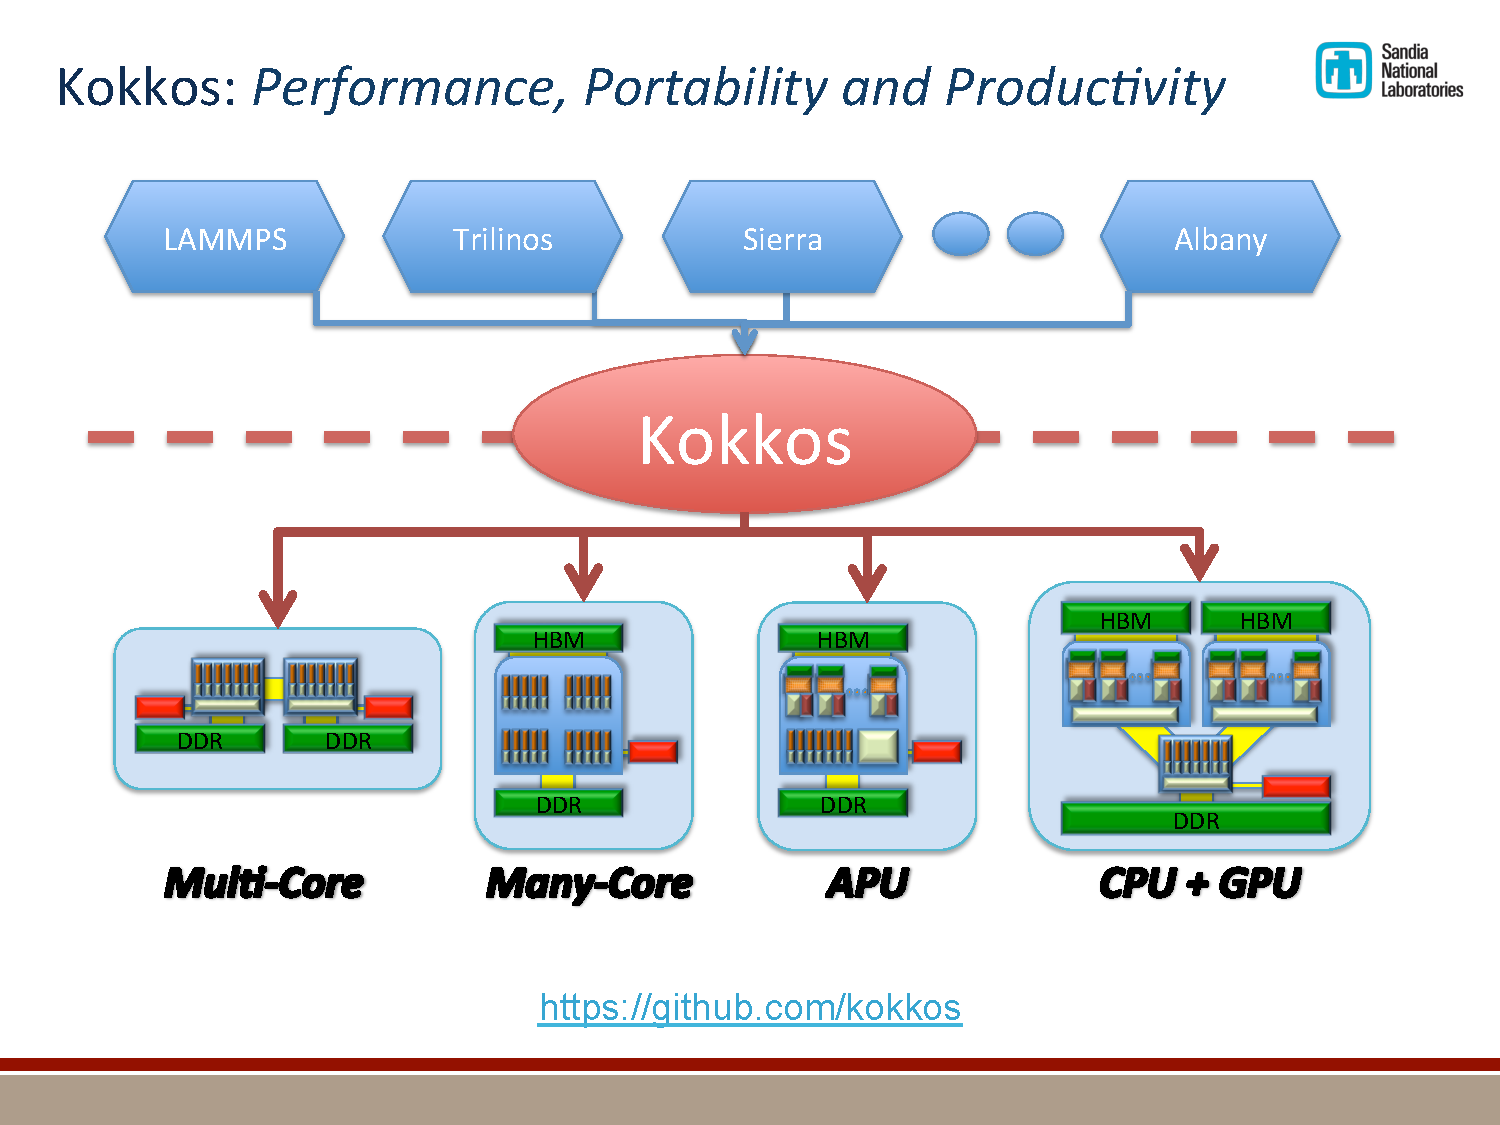
\includegraphics[width=6cm]{images/Kokkos-Multi-CoE_slide2}
  \end{center}
  
\end{frame}

%%%%%%%%%%%%%%%%%%%%%%%%%%%%%%%%%%%%%%%%%%%%%%%%%%%%%%%%%%%%%%%%%%%%%%%% 
%%%%%%%%%%%%%%%%%%%%%%%%%%%%%%%%%%%%%%%%%%%%%%%%%%%%%%%%%%%%%%%%%%%%%%%% 
\begin{frame}
  \frametitle{About Kokkos in Trilinos}

  \begin{itemize}
  \item \textbf{Build a minimal featured Trilinos with Kokkos for GPU activated} : \textcolor{red}{Tpetra + kokkos + Cuda}
    \begin{enumerate}
    \item \textbf{Example config plateform:} Ubuntu 16.04 + openmpi + cuda 8.0\\
      compiler is gcc 5.4.0
    \item \textbf{Get Trilinos sources:}\\
      \texttt{git clone https://github.com/trilinos/Trilinos.git;} \texttt{cd Trilinos; git checkout develop}
    \item \textbf{CMake configuration script:} Use the provided configuration file \texttt{configure\_tpetra\_kokkos\_cuda\_nvcc\_wrapper.sh} located in the provided archive (\texttt{doc/trilinos})\\
      this script needs slights changes (var \texttt{OMPI\_CXX} and install prefix)\\
      this script must be run in a build directory (not directly in trilinos sources).\\
      this config will build kokkos with unit tests and examples.
    \item \textbf{Build:} \texttt{make -j; make install}
    \item \textbf{Build a sample project.}
    \end{enumerate}
  \end{itemize}

\end{frame}

%%%%%%%%%%%%%%%%%%%%%%%%%%%%%%%%%%%%%%%%%%%%%%%%%%%%%%%%%%%%%%%%%%%%%%%% 
%%%%%%%%%%%%%%%%%%%%%%%%%%%%%%%%%%%%%%%%%%%%%%%%%%%%%%%%%%%%%%%%%%%%%%%% 
\begin{frame}
  \frametitle{Trilinos/Tpetra example project}

  \begin{itemize}
  \item Directory \texttt{doc/trilinos/tpetra\_example} contains a minimal example application for trilinos/tpetra. You just need to set env variable \texttt{TRILINOS\_PATH} to install directory.
  \end{itemize}
  
\end{frame}


\end{document}
